\documentclass[conference]{IEEEtran}
\IEEEoverridecommandlockouts

% ---------------------------------------------------------------------------
% Packages
% ---------------------------------------------------------------------------
\usepackage{cite}
\usepackage{amsmath,amssymb,amsfonts}
\usepackage{bm}
\usepackage{graphicx}
\usepackage{booktabs}
\usepackage{multirow}
\usepackage{xcolor}
\usepackage{tikz}
\usetikzlibrary{positioning,arrows.meta,calc,fit,backgrounds}
\usepackage{pgfplots}
\pgfplotsset{compat=1.18}
\usepgfplotslibrary{groupplots}
\usepackage[hidelinks]{hyperref}

% Condition colours used consistently across all figures
\definecolor{cGlocal}{RGB}{31,119,180}
\definecolor{cHmlm}{RGB}{214,39,40}
\definecolor{cNone}{RGB}{127,127,127}
\definecolor{cAux}{RGB}{44,160,44}

\newcommand{\glocal}{\textsc{GlocalDoc}}
\newcommand{\hmlm}{\mbox{H-MLM}}

% --- Palette and node styles for the architecture figure (Fig. 1) ---
\definecolor{tBlue}   {RGB}{52,119,196}
\definecolor{sGreen}  {RGB}{56,142,60}
\definecolor{ibOrange}{RGB}{230,130,30}
\definecolor{lossRed} {RGB}{198,40,40}
\definecolor{pPurple} {RGB}{123,31,162}
\definecolor{eGold}   {RGB}{180,140,0}
\definecolor{uwBrown} {RGB}{120,80,40}
\tikzset{
  nd/.style  = {draw, rounded corners=4pt, align=center, inner sep=5pt,
                minimum width=3.0cm, minimum height=0.9cm, font=\small},
  T/.style   = {nd, draw=tBlue,   fill=tBlue!10},
  S/.style   = {nd, draw=sGreen,  fill=sGreen!10},
  ENC/.style = {nd, draw=eGold,   fill=eGold!15},
  IB/.style  = {nd, draw=ibOrange,fill=ibOrange!18},
  PL/.style  = {nd, draw=pPurple, fill=pPurple!12},
  PRED/.style= {nd, draw=pPurple!80, fill=pPurple!7, densely dotted,
                minimum width=2.2cm, minimum height=0.85cm},
  DR/.style  = {nd, draw=sGreen!70, fill=sGreen!4, densely dashed},
  LO/.style  = {nd, draw=lossRed, fill=lossRed!10, minimum width=2.8cm},
  LOX/.style = {nd, draw=lossRed, fill=lossRed!10, minimum width=3.0cm,
                double, double distance=1pt},
  TOT/.style = {nd, draw=uwBrown, fill=uwBrown!8, font=\small},
  Tarr/.style ={-{Stealth[length=5pt]}, thick, tBlue!60,  dashed},
  Sarr/.style ={-{Stealth[length=5pt]}, thick, sGreen!70},
  Larr/.style ={-{Stealth[length=4pt]}, thick, lossRed},
  EMA/.style  ={-{Stealth[length=5pt]}, thick, ibOrange!80, dashed},
}

\begin{document}

\title{GlocalDoc: A Global and Local Information Bottleneck\\ for Few-Shot Legal Document Representation}

\author{%
\IEEEauthorblockN{Brando Mattivi}
\IEEEauthorblockA{Faculty of Engineering\\
Free University of Bozen-Bolzano, Italy\\
\texttt{brandomattivi@gmail.com}}
\and
\IEEEauthorblockN{Roger Feliu}
\IEEEauthorblockA{Faculty of Engineering\\
Free University of Bozen-Bolzano, Italy}}

\maketitle

% ---------------------------------------------------------------------------
% Abstract
% ---------------------------------------------------------------------------
\begin{abstract}
Modern language models produce contextual embeddings that capture local meaning
with remarkable accuracy, yet they tend to lose track of a document considered as
a whole. The limitation is acute for long and highly structured texts such as
legal judgments, where the decisive signal is spread across many paragraphs. We
present \glocal{}, a pre-training framework that trains a paragraph-level encoder
to produce document embeddings reflecting both local content and global structure.
\glocal{} couples a teacher-student architecture with an information bottleneck: a
momentum teacher encodes the clean document, a student encodes a corrupted view,
and a learned bottleneck compresses the pooled student representation while three
alignment objectives match it to the teacher at the paragraph, partial-document,
and full-document level. We evaluate \glocal{} against a hierarchical masked
language model baseline (\hmlm{}) and an unpretrained baseline on few-shot
multi-label classification of European Court of Human Rights cases. Our working
hypothesis was that a more global embedding should help most when supervision is
scarce. The evidence supports this only in the extreme regime. With ten labelled
examples per class \glocal{} attains the best macro-F1 and, more tellingly, the
lowest variance across seeds, while the masked language model often fails to learn
at all. Once fifty or more examples per class are available the ordering reverses
and \hmlm{} dominates. The bottleneck therefore behaves as a strong prior that is
valuable under scarcity but discards lexical detail that becomes useful with more
data. We also report a representational collapse specific to corpora with heavy
boilerplate, and show that centring the teacher target removes it.
\end{abstract}

\begin{IEEEkeywords}
information bottleneck, self-distillation, document representation, few-shot
learning, legal NLP, representational collapse.
\end{IEEEkeywords}

% ---------------------------------------------------------------------------
\section{Introduction}
% ---------------------------------------------------------------------------
Pre-trained transformer encoders have made the local semantics of text easy to
recover. A model such as RoBERTa \cite{liu2019roberta} assigns nearly synonymous
sentences nearly identical vectors, and this property underpins most retrieval and
classification systems in production. The same models are far less reliable when
the unit of interest is an entire long document. A single forward pass is bounded
by a context window of a few hundred tokens, and the common workaround of encoding
a truncated prefix throws away most of the text. Pooling sentence vectors recovers
coverage but not structure, because mean or maximum pooling treats a judgment as a
bag of paragraphs and ignores how the parts compose into a decision.

Legal text makes the problem concrete. A European Court of Human Rights (ECtHR)
judgment states facts across dozens of numbered paragraphs, and the articles that
were allegedly violated depend on the interaction of those paragraphs rather than
on any one of them. Annotating such documents is expensive and requires expert
knowledge, so the realistic setting is few-shot: a handful of labelled cases per
article, not thousands. A representation that already encodes the global shape of a
document, before any task labels are seen, should transfer better to this regime
than one tuned only for token-level prediction.

We study whether an explicit compression objective can produce such a
representation. The information bottleneck principle \cite{tishby2000information}
prescribes keeping the part of an input that is predictive of a target while
discarding the rest, and its variational form \cite{alemi2017deep} makes the idea
trainable inside a neural network. We instantiate it for documents in a framework
we call \glocal{}. A student encoder reads a corrupted view of a judgment and pools
it into a single vector through a stochastic bottleneck; a momentum teacher reads
the clean judgment; and the student is trained to predict the teacher at three
granularities while paying a compression cost on the bottleneck. The design
borrows the asymmetry of non-contrastive self-distillation
\cite{grill2020bootstrap,chen2021exploring}, which is what prevents the encoder
from satisfying the alignment objectives with a constant output.

We compare \glocal{} to \hmlm{}, a hierarchical masked language model in the spirit
of SMITH \cite{yang2020beyond} that keeps the same encoder and the same document
pooler but replaces compression and alignment with token reconstruction plus a
single pooling target. Both are evaluated by freezing the pre-trained encoder, then
fine-tuning a linear classifier on $N \in \{10, 50, 100\}$ labelled cases per
article. The questions we set out to answer are the following.

\begin{itemize}
\item \textbf{RQ1.} Does global and local bottleneck pre-training yield better
few-shot document features than hierarchical masked language modelling?
\item \textbf{RQ2.} How does any advantage depend on the amount of supervision
available at fine-tuning time?
\item \textbf{RQ3.} What training instabilities does the objective introduce on a
boilerplate-heavy corpus, and which mechanisms resolve them?
\end{itemize}

The contributions of the paper follow these questions. We describe the \glocal{}
objective and the stabilisation mechanisms it needs in practice. We report a
controlled comparison in which the only variable is the pre-training objective, and
we find a clear interaction with $N$: \glocal{} wins at $N=10$ and \hmlm{} wins from
$N=50$ onward. We show that the most useful property of \glocal{} at $N=10$ is not
a large mean improvement but a sharp reduction in seed variance, where the baseline
collapses to zero on several seeds. Finally we document a failure mode that is easy
to overlook on natural images but severe on legal text: when documents are nearly
identical in the encoder's initial embedding space, the teacher target degenerates
to a constant, and centring it in the style of DINO \cite{caron2021emerging}
restores a usable training signal.

% ---------------------------------------------------------------------------
\section{Related Work}
% ---------------------------------------------------------------------------

\subsection{Information bottleneck and variational compression}
The information bottleneck frames representation learning as a trade-off between
keeping information about a target and compressing the input
\cite{tishby2000information,tishby2015deep}. The deep variational bottleneck makes
this practical by parameterising a stochastic encoder and bounding the mutual
information terms \cite{alemi2017deep}, which connects it directly to the
variational autoencoder \cite{kingma2014auto} and to $\beta$-VAE
\cite{higgins2017beta}, where a weight on the Kullback-Leibler term controls the
strength of compression. A recurring difficulty is posterior collapse, in which the
encoder ignores the input and the bottleneck reverts to its prior. The free-bits
heuristic \cite{kingma2016improved} addresses this by exempting a small budget of
information per latent dimension from the compression penalty. \glocal{} uses a
hard per-dimension form of free bits together with a warm-up on $\beta$, so that
compression is introduced only after the alignment objectives have shaped the
representation.

\subsection{Non-contrastive self-distillation}
Self-supervised methods that align two views of an input without negative pairs
must avoid the trivial solution of a constant embedding. BYOL \cite{grill2020bootstrap}
and SimSiam \cite{chen2021exploring} achieve this with an asymmetric design: a
predictor network on one branch, a stop-gradient on the other, and in BYOL a slow
moving-average (momentum) teacher in the lineage of MoCo \cite{he2020momentum}.
DINO \cite{caron2021emerging} adds centring and sharpening of the teacher output to
keep it from concentrating on a single direction. VICReg \cite{bardes2022vicreg}
and Barlow Twins \cite{zbontar2021barlow} take a complementary route and prevent
collapse explicitly by regularising the variance and the cross-correlation of the
embeddings. \glocal{} combines these ideas rather than choosing among them, because
on our corpus each one alone proved insufficient, a point we return to in
Section~\ref{sec:results} and Appendix~\ref{app:collapse}.

\subsection{Masked language models and long documents}
BERT \cite{devlin2019bert} and RoBERTa \cite{liu2019roberta} established masked
language modelling as the dominant pre-training objective for encoders, and
DistilRoBERTa \cite{sanh2019distilbert} provides a compact six-layer version that we
adopt as the shared backbone. None of these handle long documents natively.
Longformer \cite{beltagy2020longformer} extends the context window with sparse
attention, whereas hierarchical models such as SMITH \cite{yang2020beyond} encode
sentences or paragraphs independently and compose them with a second-level module.
Our \hmlm{} baseline is hierarchical in this sense: it encodes each paragraph,
trains an attention pooler to reconstruct the document from a partial view, and
keeps token-level masked prediction as an auxiliary loss.

\subsection{Legal NLP and few-shot classification}
LexGLUE \cite{chalkidis2022lexglue} collects several legal benchmarks, including the
ECtHR allegation task derived from earlier work on judgment prediction
\cite{chalkidis2019neural}. The task is multi-label and strongly imbalanced, which
makes macro-averaged F1 the appropriate primary metric. Few-shot text
classification has been studied extensively for in-context learning with large
decoders \cite{brown2020language}, but the encoder-plus-linear-head setting we use
isolates the quality of the pre-trained representation from any prompting effect.
Document and sentence embedding methods such as Sentence-BERT
\cite{reimers2019sentence} and SimCSE \cite{gao2021simcse} optimise pooled vectors
directly, yet they target short inputs and do not model paragraph structure, which
is the gap \glocal{} addresses.

\subsection{Balancing multiple objectives}
\glocal{} optimises four losses at once. Rather than searching for fixed weights we
use homoscedastic uncertainty weighting \cite{kendall2018multi}, which treats each
loss as a Gaussian likelihood with a learned observation noise and produces
self-tuning weights. We keep the anti-collapse regularisers outside this mechanism,
since a signal whose purpose is to prevent degeneracy must not be down-weighted by
the same optimiser that benefits from degeneracy.

% ---------------------------------------------------------------------------
% Architecture figure (full width)
% ---------------------------------------------------------------------------
\begin{figure*}[p]
\centering
\resizebox{0.95\textwidth}{!}{%
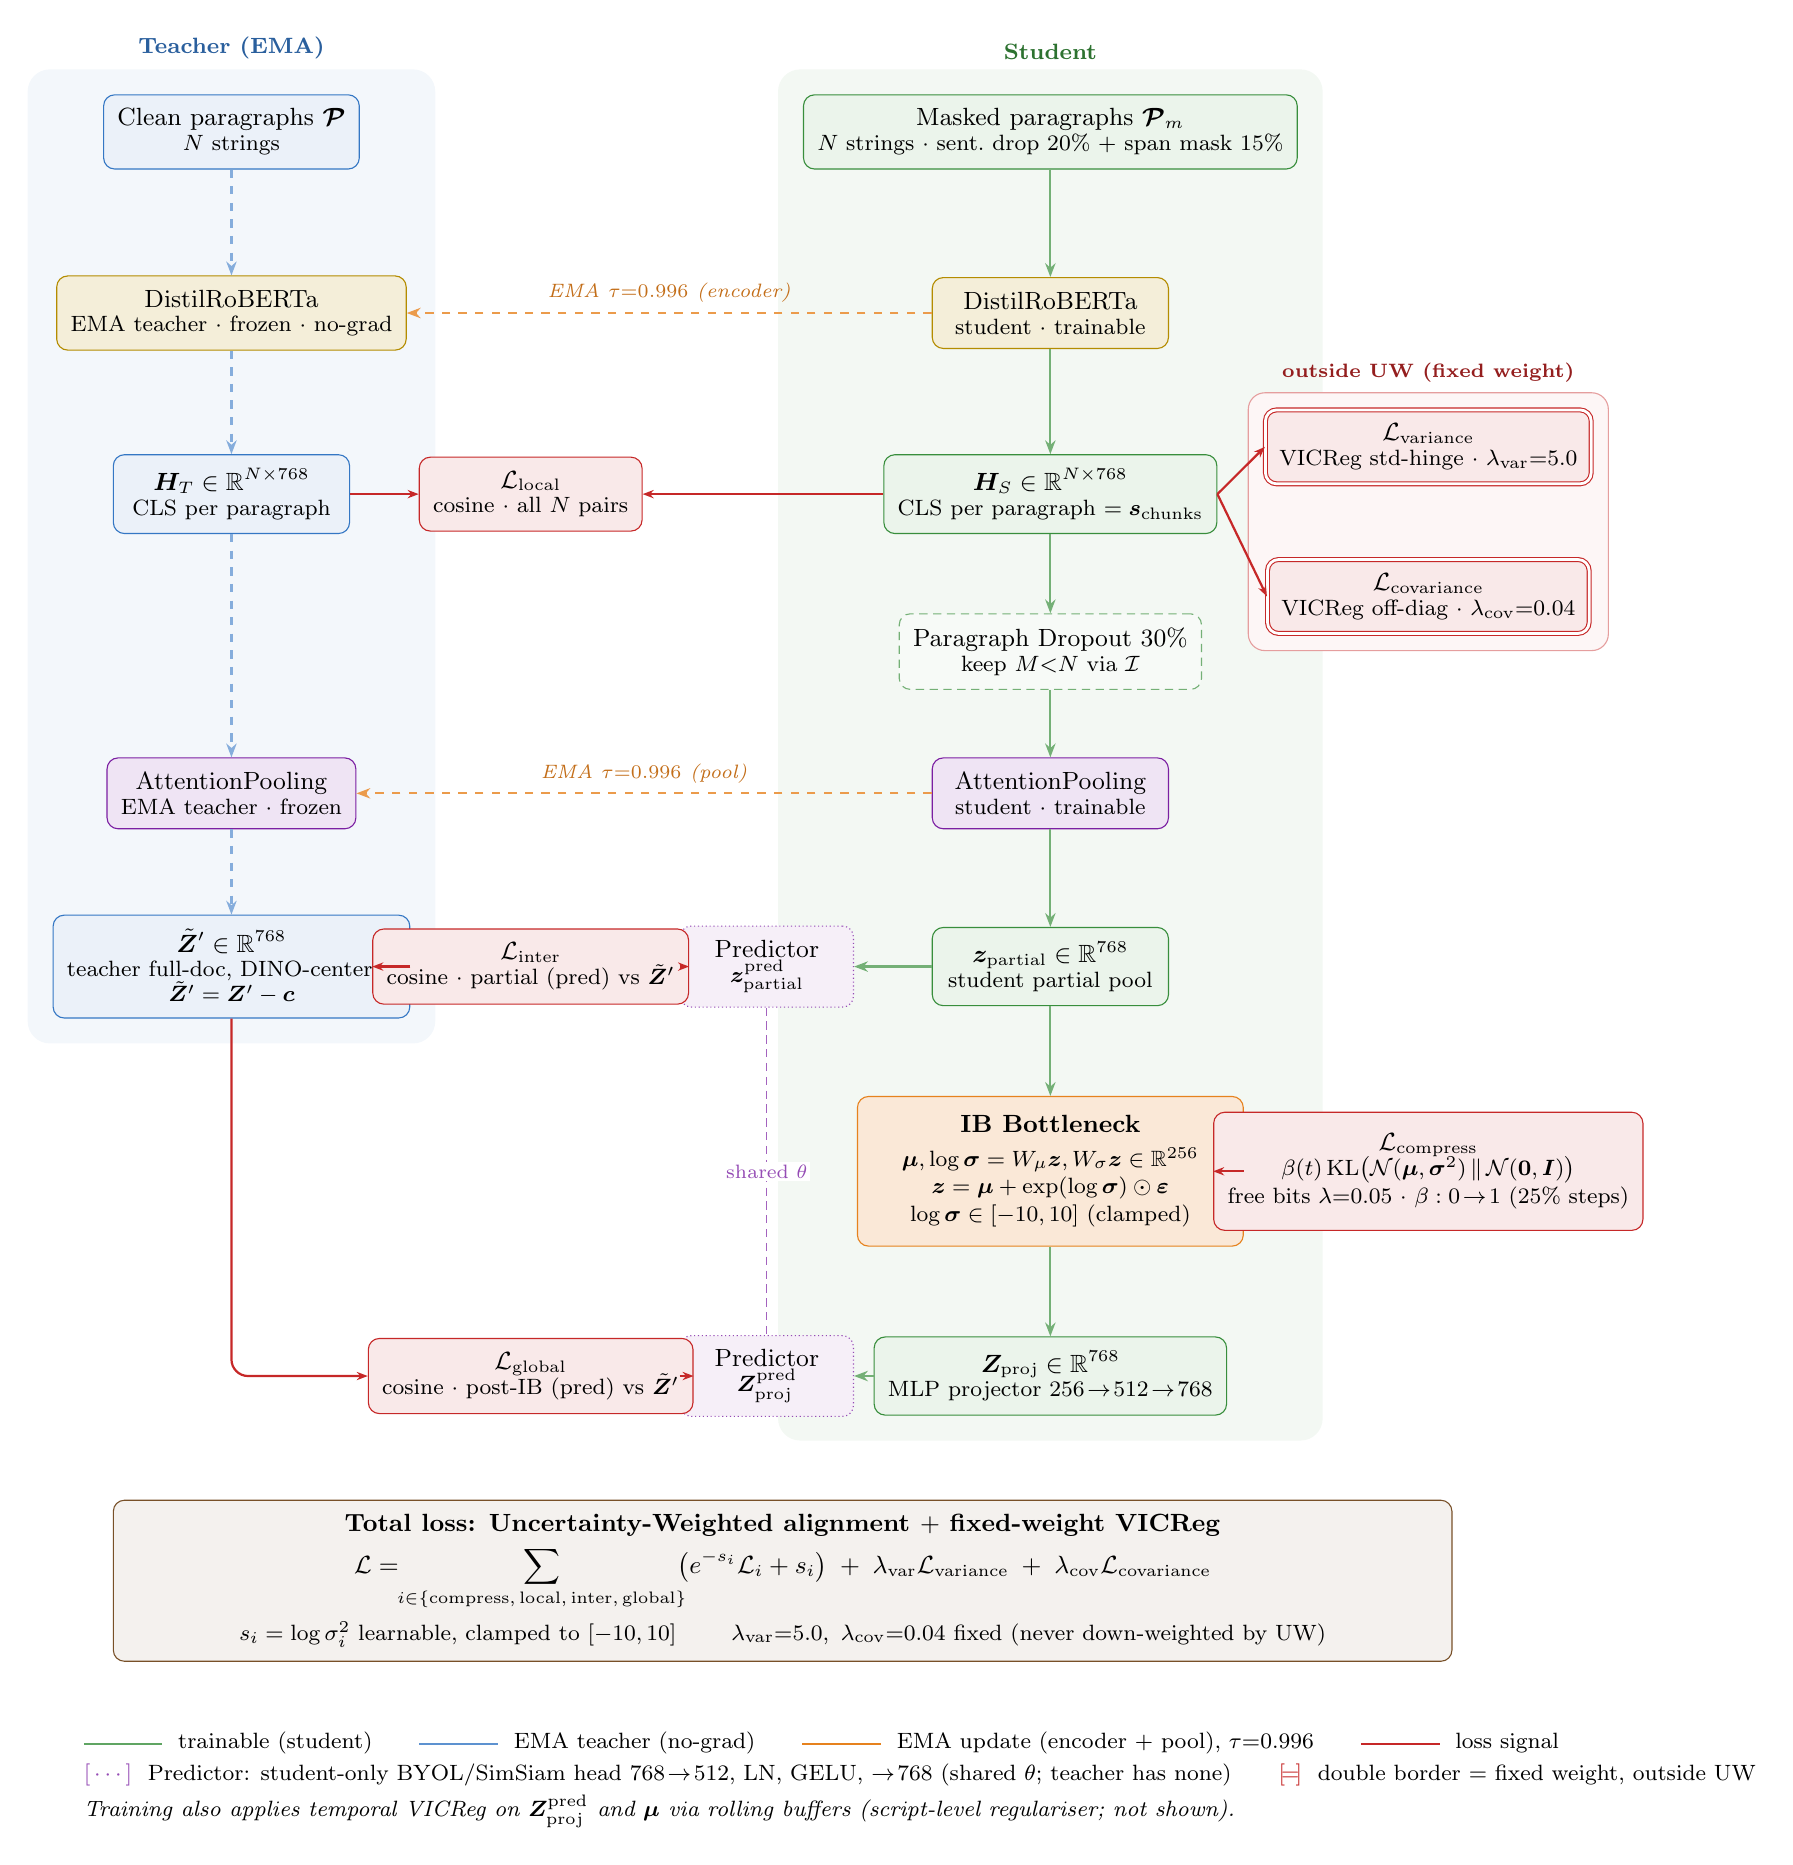
\begin{tikzpicture}

%% TEACHER branch (x = 0): separate frozen EMA encoder
\node[T]   (t_in)  at (0,   0   ) {Clean paragraphs $\bm{\mathcal{P}}$\\[-2pt]\footnotesize $N$ strings};
\node[ENC] (t_enc) at (0,  -2.3 ) {DistilRoBERTa\\[-2pt]\footnotesize EMA teacher $\cdot$ frozen $\cdot$ no-grad};
\node[T]   (t_cls) at (0,  -4.6 ) {$\bm{H}_T\in\mathbb{R}^{N\times768}$\\[-2pt]\footnotesize CLS per paragraph};
\node[PL]  (t_pl)  at (0,  -8.4 ) {AttentionPooling\\[-2pt]\footnotesize EMA teacher $\cdot$ frozen};
\node[T, minimum width=3.2cm]
           (t_zt)  at (0, -10.6 ) {$\tilde{\bm{Z}}'\in\mathbb{R}^{768}$\\[-2pt]\footnotesize teacher full-doc, DINO-centered\\[-2pt]\footnotesize $\tilde{\bm{Z}}'=\bm{Z}'-\bm{c}$};

\draw[Tarr] (t_in)  -- (t_enc);
\draw[Tarr] (t_enc) -- (t_cls);
\draw[Tarr] (t_cls) -- (t_pl);
\draw[Tarr] (t_pl)  -- (t_zt);

%% STUDENT branch (x = 10.4): trainable
\node[S, minimum width=3.6cm]
           (s_in)  at (10.4,   0   ) {Masked paragraphs $\bm{\mathcal{P}}_m$\\[-2pt]\footnotesize $N$ strings $\cdot$ sent.\ drop $20\%$ $+$ span mask $15\%$};
\node[ENC] (s_enc) at (10.4,  -2.3 ) {DistilRoBERTa\\[-2pt]\footnotesize student $\cdot$ trainable};
\node[S, minimum width=3.6cm]
           (s_cls) at (10.4,  -4.6 ) {$\bm{H}_S\in\mathbb{R}^{N\times768}$\\[-2pt]\footnotesize CLS per paragraph $=\bm{s}_{\mathrm{chunks}}$};
\node[DR]  (s_dr)  at (10.4,  -6.6 ) {Paragraph Dropout $30\%$\\[-2pt]\footnotesize keep $M{<}N$ via $\mathcal{I}$};
\node[PL]  (s_pl)  at (10.4,  -8.4 ) {AttentionPooling\\[-2pt]\footnotesize student $\cdot$ trainable};
\node[S]   (s_zp)  at (10.4, -10.6 ) {$\bm{z}_{\mathrm{partial}}\in\mathbb{R}^{768}$\\[-2pt]\footnotesize student partial pool};
\node[IB, minimum width=4.9cm, minimum height=1.9cm]
           (s_ib)  at (10.4, -13.2 ) {\textbf{IB Bottleneck}\\[1pt]
                 \footnotesize $\bm{\mu},\log\bm{\sigma}=W_\mu\bm{z},W_\sigma\bm{z}\in\mathbb{R}^{256}$\\[-1pt]
                 \footnotesize $\bm{z}=\bm{\mu}+\exp(\log\bm{\sigma})\odot\bm{\varepsilon}$\\[-1pt]
                 \footnotesize $\log\bm{\sigma}\in[-10,10]$ (clamped)};
\node[S, minimum width=3.6cm]
           (s_zj)  at (10.4, -15.8 ) {$\bm{Z}_{\mathrm{proj}}\in\mathbb{R}^{768}$\\[-2pt]\footnotesize MLP projector $256\!\to\!512\!\to\!768$};

\draw[Sarr] (s_in)  -- (s_enc);
\draw[Sarr] (s_enc) -- (s_cls);
\draw[Sarr] (s_cls) -- (s_dr);
\draw[Sarr] (s_dr)  -- (s_pl);
\draw[Sarr] (s_pl)  -- (s_zp);
\draw[Sarr] (s_zp)  -- (s_ib);
\draw[Sarr] (s_ib)  -- (s_zj);

%% Student-only PREDICTOR (inline, shared weights)
\node[PRED] (p_a) at (6.8, -10.6) {Predictor\\[-2pt]\footnotesize $\bm{z}_{\mathrm{partial}}^{\mathrm{pred}}$};
\node[PRED] (p_b) at (6.8, -15.8) {Predictor\\[-2pt]\footnotesize $\bm{Z}_{\mathrm{proj}}^{\mathrm{pred}}$};
\draw[Sarr] (s_zp.west) -- (p_a.east);
\draw[Sarr] (s_zj.west) -- (p_b.east);
\draw[densely dashed, pPurple!70] (p_a.south) -- (p_b.north)
      node[midway, fill=white, inner sep=1pt, font=\scriptsize, text=pPurple!80]{shared $\theta$};

%% LOSS SPINE (x = 3.8): each loss between its operands
\node[LO] (l_loc) at (3.8,  -4.6) {$\mathcal{L}_{\mathrm{local}}$\\[-2pt]\footnotesize cosine $\cdot$ all $N$ pairs};
\draw[Larr] (t_cls.east) -- (l_loc.west);
\draw[Larr] (s_cls.west) -- (l_loc.east);

\node[LO] (l_int) at (3.8, -10.6) {$\mathcal{L}_{\mathrm{inter}}$\\[-2pt]\footnotesize cosine $\cdot$ partial (pred) vs $\tilde{\bm{Z}}'$};
\draw[Larr] (t_zt.east) -- (l_int.west);
\draw[Larr] (p_a.west)  -- (l_int.east);

\node[LO] (l_glb) at (3.8, -15.8) {$\mathcal{L}_{\mathrm{global}}$\\[-2pt]\footnotesize cosine $\cdot$ post-IB (pred) vs $\tilde{\bm{Z}}'$};
\draw[Larr] (p_b.west) -- (l_glb.east);
\draw[Larr, rounded corners=6pt] (t_zt.south) |- (l_glb.west);

%% REGULARIZERS (x = 15.2): beside their source
\node[LO, minimum width=3.0cm, minimum height=1.5cm]
      (l_cmp) at (15.2, -13.2) {$\mathcal{L}_{\mathrm{compress}}$\\[-2pt]
            \footnotesize $\beta(t)\,\mathrm{KL}\bigl(\mathcal{N}(\bm{\mu},\bm{\sigma}^2)\,\|\,\mathcal{N}(\bm{0},\bm{I})\bigr)$\\[-1pt]
            \footnotesize free bits $\lambda{=}0.05$ $\cdot$ $\beta:0\!\to\!1$ (25\% steps)};
\draw[Larr] (s_ib.east) -- (l_cmp.west);

\node[LOX] (l_var) at (15.2,  -4.0) {$\mathcal{L}_{\mathrm{variance}}$\\[-2pt]\footnotesize VICReg std-hinge $\cdot$ $\lambda_{\mathrm{var}}{=}5.0$};
\node[LOX] (l_cov) at (15.2,  -5.9) {$\mathcal{L}_{\mathrm{covariance}}$\\[-2pt]\footnotesize VICReg off-diag $\cdot$ $\lambda_{\mathrm{cov}}{=}0.04$};
\draw[Larr] (s_cls.east) -- (l_var.west);
\draw[Larr] (s_cls.east) -- (l_cov.west);

%% EMA links (student -> teacher): encoder AND pool
\draw[EMA] (s_enc.west) -- (t_enc.east)
      node[midway, above, font=\scriptsize\itshape, text=ibOrange!85!black]{EMA $\tau{=}0.996$ (encoder)};
\draw[EMA] (s_pl.west) -- (t_pl.east)
      node[midway, above, font=\scriptsize\itshape, text=ibOrange!85!black]{EMA $\tau{=}0.996$ (pool)};

%% TOTAL LOSS
\node[TOT, minimum width=17cm, minimum height=2.0cm, align=center]
      (l_tot) at (7.0, -18.4) {%
      \textbf{Total loss: Uncertainty-Weighted alignment $+$ fixed-weight VICReg}\\[3pt]
      $\displaystyle \mathcal{L}=\!\!\sum_{i\in\{\mathrm{compress},\,\mathrm{local},\,\mathrm{inter},\,\mathrm{global}\}}\!\!\bigl(e^{-s_i}\mathcal{L}_i+s_i\bigr)\;+\;\lambda_{\mathrm{var}}\mathcal{L}_{\mathrm{variance}}\;+\;\lambda_{\mathrm{cov}}\mathcal{L}_{\mathrm{covariance}}$\\[3pt]
      \footnotesize $s_i=\log\sigma_i^{2}$ learnable, clamped to $[-10,10]$ \qquad
      $\lambda_{\mathrm{var}}{=}5.0,\ \lambda_{\mathrm{cov}}{=}0.04$ fixed (never down-weighted by UW)};

%% BACKGROUND PANELS (fit, auto-sized)
\begin{scope}[on background layer]
  \node[fill=tBlue!6, rounded corners=8pt, fit=(t_in)(t_enc)(t_cls)(t_pl)(t_zt), inner sep=9pt] (tpanel){};
  \node[fill=sGreen!6, rounded corners=8pt, fit=(s_in)(s_enc)(s_cls)(s_dr)(s_pl)(s_zp)(s_ib)(s_zj), inner sep=9pt] (spanel){};
  \node[draw=lossRed!45, fill=lossRed!4, rounded corners=6pt, fit=(l_var)(l_cov), inner sep=6pt] (uwbox){};
\end{scope}
\node[font=\bfseries\footnotesize, text=tBlue!80!black, anchor=south] at (tpanel.north) {Teacher (EMA)};
\node[font=\bfseries\footnotesize, text=sGreen!80!black, anchor=south] at (spanel.north) {Student};
\node[font=\bfseries\scriptsize, text=lossRed!75!black, anchor=south] at (uwbox.north) {outside UW (fixed weight)};

%% LEGEND
\node[font=\footnotesize, anchor=north west, align=left] at (-2.0,-20.2) {%
  \textcolor{sGreen!80}{\rule[0.4ex]{1.0cm}{0.7pt}}~ trainable (student)\qquad
  \textcolor{tBlue!80}{\rule[0.4ex]{1.0cm}{0.7pt}}~ EMA teacher (no-grad)\qquad
  \textcolor{ibOrange}{\rule[0.4ex]{1.0cm}{0.7pt}}~ EMA update (encoder $+$ pool), $\tau{=}0.996$\qquad
  \textcolor{lossRed}{\rule[0.4ex]{1.0cm}{0.7pt}}~ loss signal\\[2pt]
  \textcolor{pPurple!80}{$[\,\cdots\,]$}~ Predictor: student-only BYOL/SimSiam head $768\!\to\!512$, LN, GELU, $\to\!768$ (shared $\theta$; teacher has none)\qquad
  \textcolor{lossRed}{$[\!=\!]$}~ double border $=$ fixed weight, outside UW\\[2pt]
  \textit{Training also applies temporal VICReg on $\bm{Z}_{\mathrm{proj}}^{\mathrm{pred}}$ and $\bm{\mu}$ via rolling buffers (script-level regulariser; not shown).}};

\end{tikzpicture}}
\caption{The \glocal{} architecture. The teacher branch (left, blue) is a frozen
exponential moving average of the student: it encodes the clean paragraphs with
DistilRoBERTa, pools them, and centres the full-document target as
$\tilde{\bm{Z}}'=\bm{Z}'-\bm{c}$ to remove the constant boilerplate direction. The
student branch (right, green) encodes a masked view, drops $30\%$ of paragraphs at
the pooling stage, compresses the partial pool through the information bottleneck,
and projects it back to $\mathbb{R}^{768}$. A single student-only BYOL/SimSiam
predictor with shared weights $\theta$ is applied to both the partial pool and the
projected code. The loss spine (centre) holds the three cosine alignment terms,
$\mathcal{L}_{\mathrm{local}}$ between paragraph matrices and
$\mathcal{L}_{\mathrm{inter}},\mathcal{L}_{\mathrm{global}}$ against the centred
teacher target, together with the compression term
$\mathcal{L}_{\mathrm{compress}}$, all balanced by uncertainty weighting. The
VICReg variance and covariance regularisers (right) act on the student paragraph
vectors with fixed weights, outside the uncertainty-weighted sum. Temporal VICReg
on $\bm{Z}_{\mathrm{proj}}^{\mathrm{pred}}$ and $\bm{\mu}$ is applied at the script
level and omitted here.}
\label{fig:arch}
\end{figure*}

% ---------------------------------------------------------------------------
\section{The GlocalDoc Framework}
\label{sec:method}
% ---------------------------------------------------------------------------
Figure~\ref{fig:arch} summarises the architecture. We first fix notation, then
describe the encoder, the two-level masking, the bottleneck, the alignment losses,
and the mechanisms that keep training stable.

\subsection{Notation and hierarchical encoding}
A document is a sequence of paragraphs $x = (p_1, \dots, p_N)$ with
$5 \le N \le 50$. Each paragraph is encoded independently by a shared transformer
$f_\theta$, taking the \texttt{[CLS]} representation as the paragraph vector.
Paragraphs longer than $510$ tokens are split into non-overlapping sub-chunks, each
encoded separately, and their \texttt{[CLS]} vectors are averaged, so that a
paragraph of any length maps to one vector in $\mathbb{R}^{768}$. Stacking gives the
paragraph matrix $S = [s_1; \dots; s_N] \in \mathbb{R}^{N \times 768}$.

A document vector is produced by an attention pooler
\begin{equation}
a_i = \frac{\exp(q^\top (s_i + e_i))}{\sum_{j} \exp(q^\top (s_j + e_j))}, \quad
\mathrm{pool}(S) = \sum_i a_i (s_i + e_i),
\end{equation}
where $q$ is a learned query and $e_i$ are learned positional embeddings. The
positional embeddings are initialised to zero, so the pooler begins as exact mean
pooling and departs from it only as training requires.

\subsection{Two-level masking}
\glocal{} corrupts the input at two independent levels. At the text level, each
paragraph is masked before being read by the student: sentences are dropped with
probability $0.20$, and within the surviving text spans of three to five words are
replaced by a single mask token until about $15\%$ of words are covered. At the
structural level, a paragraph dropout removes $30\%$ of paragraphs, but only at the
pooling stage. The student encoder still sees all $N$ masked paragraphs; the dropout
selects a subset of the resulting vectors before pooling, which yields a partial
view $z_{\mathrm{partial}} = \mathrm{pool}(S_{\mathrm{kept}})$. Keeping all $N$
paragraphs in the encoder is required so that the paragraph-level objective can
compare student and teacher vectors position by position.

\subsection{Information bottleneck}
The partial document vector is passed through a stochastic bottleneck. Two linear
heads produce a mean and a log standard deviation, and a latent code is sampled with
the reparameterisation trick,
\begin{equation}
\mu = W_\mu z_{\mathrm{partial}}, \quad
\log\sigma = \mathrm{clip}(W_\sigma z_{\mathrm{partial}}, -10, 10),
\end{equation}
\begin{equation}
z = \mu + \sigma \odot \varepsilon, \quad \varepsilon \sim \mathcal{N}(0, I),
\end{equation}
with $z \in \mathbb{R}^{256}$. A two-layer projector $g$ maps $z$ back to
$\mathbb{R}^{768}$, giving $Z_{\mathrm{proj}} = g(z)$. The compression cost is the
Kullback-Leibler divergence to a standard normal prior, computed in closed form and
floored per dimension by a free-bits budget $\lambda$,
\begin{equation}
\mathcal{L}_{\mathrm{compress}} = \beta_t \sum_{j=1}^{256}
\max\!\Big(\lambda,\ \tfrac{1}{2}\big(\mu_j^2 + \sigma_j^2 - 1 - 2\log\sigma_j\big)\Big).
\end{equation}
The clip on $\log\sigma$ keeps the term finite under bfloat16. The weight $\beta_t$
follows a linear warm-up from zero to one over the first quarter of training, which
lets the alignment objectives organise the representation before compression starts
to bite. We use $\lambda = 0.05$ nats per dimension. A larger floor was tried and
rejected: at $\lambda = 0.5$ the $128$-nat floor dominated the objective and forced
the mean toward a fixed magnitude regardless of the input, which is the opposite of
the intended behaviour.

\subsection{Multi-granularity alignment}
The teacher is a momentum copy of the encoder and pooler, never updated by gradient.
It reads the clean document and produces a full-document target
$Z' = \mathrm{pool}_{\mathrm{T}}(S_{\mathrm{T}})$, which is centred as described
below. Writing $\mathrm{sg}$ for stop-gradient, $h$ for the predictor, and
$d(u,v) = 1 - \cos(u,v)$ for the cosine distance, the three alignment losses are
\begin{align}
\mathcal{L}_{\mathrm{local}} &= d\big(S,\ \mathrm{sg}(S_{\mathrm{T}})\big), \\
\mathcal{L}_{\mathrm{inter}} &= d\big(h(z_{\mathrm{partial}}),\ \mathrm{sg}(Z')\big), \\
\mathcal{L}_{\mathrm{global}} &= d\big(h(Z_{\mathrm{proj}}),\ \mathrm{sg}(Z')\big).
\end{align}
The local term matches every student paragraph vector to the corresponding teacher
paragraph vector. The intermediate term asks the partial pooled view to predict the
full document before compression, and the global term asks the compressed and
projected code to predict the same target after compression. Both document-level
terms regress onto a single teacher vector, so the bottleneck must preserve whatever
is needed to reconstruct the global representation from a partial and corrupted
input.

\subsection{Preventing collapse}
The predictor $h$ is applied to the student branch only. This asymmetry, together
with the stop-gradient on the teacher, is the formal mechanism that removes the
constant-output fixed point in non-contrastive self-distillation
\cite{grill2020bootstrap,chen2021exploring}. The teacher tracks the student through
an exponential moving average with rate $\tau = 0.996$, applied to both encoder and
pooler after every optimiser step; running statistics in normalisation layers are
copied rather than averaged, since averaging them drifts away from the student's
activation distribution.

On its own the asymmetry was not enough on legal text. We add the variance and
covariance regularisers of VICReg \cite{bardes2022vicreg} on the student paragraph
vectors,
\begin{equation}
V(S) = \tfrac{1}{d}\sum_{j} \max\!\big(0,\ \gamma - \sqrt{\mathrm{Var}(S_{\cdot j}) + \epsilon}\big),
\end{equation}
\begin{equation}
C(S) = \tfrac{1}{d}\sum_{i \ne j} \big[\mathrm{Cov}(S)\big]_{ij}^2,
\end{equation}
with the variance hinge $\gamma = 0.5$. Because per-document paragraph statistics do
not see across-document variation, we add the same two regularisers in a temporal
form on the post-predictor document code and on the bottleneck mean, computed
against a rolling buffer of the sixteen most recent samples whose gradient is
detached. These temporal terms penalise a representation that is constant across
consecutive documents even when it varies within a document.

The remaining and most important fix concerns the teacher target itself. ECtHR
judgments share a large amount of boilerplate, and in the encoder's initial space
the documents are nearly indistinguishable: a probe over $200$ documents found a
median pairwise cosine of $0.9997$, with every ordered pair above $0.99$. A teacher
target that is almost constant across documents lets the predictor satisfy
$\mathcal{L}_{\mathrm{inter}}$ and $\mathcal{L}_{\mathrm{global}}$ by emitting that
constant. We remove this fixed point with DINO-style centring
\cite{caron2021emerging}: a running mean $c$ is maintained with momentum $0.9$ and
subtracted from the teacher output,
\begin{equation}
Z'_{\mathrm{c}} = Z' - c, \qquad
c \leftarrow 0.9\,c + 0.1\,\overline{Z'}_{\mathrm{batch}}.
\end{equation}
The centred vector is the actual regression target. Section~\ref{sec:results} shows
that this single change is what keeps training stable.

\subsection{Objective and optimisation}
The four primary losses are combined by homoscedastic uncertainty weighting
\cite{kendall2018multi} with learned log-variances
$s = (s_{\mathrm{c}}, s_{\mathrm{l}}, s_{\mathrm{i}}, s_{\mathrm{g}})$,
\begin{equation}
\mathcal{L}_{\mathrm{UW}} = \!\!\sum_{k} \big(e^{-s_k}\,\mathcal{L}_k + s_k\big),
\end{equation}
and the anti-collapse regularisers are added with fixed weights outside the weighted
sum,
\begin{equation}
\mathcal{L} = \mathcal{L}_{\mathrm{UW}} + \omega_v V(S) + \omega_c C(S)
+ \mathcal{L}_{\mathrm{temporal}}.
\end{equation}
The weights $s$ are given their own parameter group with a learning rate three
orders of magnitude larger than the encoder and no weight decay. Without this, the
gradient on $s$ is too small to move the weights away from their initialisation, and
the uncertainty weighting stays degenerate at uniform weights for the whole run.

\subsection{The H-MLM baseline}
\hmlm{} keeps the backbone, the paragraph encoding, and the attention pooler, and
removes everything specific to \glocal{}. It optimises a token-level masked language
modelling loss $\mathcal{L}_{\mathrm{mlm}}$ on each paragraph with a $15\%$ mask
rate, and a single pooling objective that asks the attention pool over a $70\%$
subset of paragraphs to predict the stop-gradient mean of all paragraph vectors,
\begin{equation}
\mathcal{L} = \tfrac{1}{2}\mathcal{L}_{\mathrm{mlm}}
+ \tfrac{1}{2}\,d\big(\mathrm{pool}(S_{\mathrm{kept}}),\ \mathrm{sg}(\overline{S})\big).
\end{equation}
There is no bottleneck, no teacher, no predictor, and no uncertainty weighting. The
comparison between \glocal{} and \hmlm{} is therefore a comparison of pre-training
objectives under an identical architecture and an identical fine-tuning procedure.

% ---------------------------------------------------------------------------
\section{Experimental Setup}
\label{sec:setup}
% ---------------------------------------------------------------------------

\subsection{Data}
We use the ECtHR Task A subset of LexGLUE \cite{chalkidis2022lexglue}, in which the
input is the list of fact paragraphs of a case and the target is the set of
allegedly violated Convention articles over ten labels. We keep documents with
between five and fifty paragraphs, which removes fewer than one percent of cases and
bounds the cost of encoding. The label distribution is severely skewed. The most
frequent article appears in roughly $4{,}700$ training cases and the rarest in about
$41$, a ratio close to one hundred. This motivates macro-averaged F1 as the primary
metric, with micro-averaged F1 reported alongside it.

\subsection{Pre-training}
Both objectives pre-train DistilRoBERTa \cite{sanh2019distilbert} on the same
filtered training split. \glocal{} runs for five epochs and \hmlm{} for three, both
with batch size one and gradient accumulation, in bfloat16 with a linear schedule
and ten percent warm-up. The full configuration is listed in
Appendix~\ref{app:hparams}, Table~\ref{tab:hparams}. We deliberately report a single
pre-training run per objective, which is a limitation we discuss in
Section~\ref{sec:discussion}.

\subsection{Fine-tuning protocol}
At fine-tuning time the pre-trained encoder and pooler are loaded into a document
classifier with a linear head over the pooled vector. For \glocal{} we load the
student pooler, since the teacher pooler is a moving average that barely departs from
its initialisation over a short run. For each condition we evaluate
$N \in \{10, 50, 100\}$ labelled cases per article, sampled with a multi-label aware
routine that keeps the per-article quota and deduplicates cases covering several
articles. Each setting is repeated over five seeds. The seed is fixed before both
the few-shot sampling and the construction of the classifier head, so that a seed
varies both the sample and the head initialisation rather than the sample alone. We
train for ten epochs with a binary cross-entropy loss over the ten labels, a cosine
schedule with ten percent warm-up, and a decision threshold of $0.5$ at evaluation.
The checkpoint with the best validation macro-F1 is evaluated on the held-out test
split.

\subsection{Baselines}
Besides \hmlm{}, we include a no-pre-training baseline that loads an off-the-shelf
DistilRoBERTa with a freshly initialised pooler. It measures how much of the
few-shot performance is attributable to pre-training at all, as opposed to the
architecture and the fine-tuning procedure.

% ---------------------------------------------------------------------------
% Main results table
% ---------------------------------------------------------------------------
\begin{table}[t]
\centering
\caption{Few-shot test results on ECtHR Task A. Mean over five seeds, standard
deviation in parentheses. Best per row block in bold; the best method at each $N$ is
the bold value within that $N$.}
\label{tab:main}
\begin{tabular}{l c c c}
\toprule
Method & $N$ & Macro-F1 & Micro-F1 \\
\midrule
\multirow{3}{*}{No pre-training}
 & 10  & 0.001 (0.001) & 0.003 (0.004) \\
 & 50  & 0.025 (0.008) & 0.077 (0.030) \\
 & 100 & 0.042 (0.013) & 0.106 (0.019) \\
\midrule
\multirow{3}{*}{\hmlm{}}
 & 10  & 0.019 (0.023) & 0.069 (0.085) \\
 & 50  & \textbf{0.273} (0.061) & \textbf{0.354} (0.060) \\
 & 100 & \textbf{0.372} (0.032) & \textbf{0.454} (0.030) \\
\midrule
\multirow{3}{*}{\glocal{}}
 & 10  & \textbf{0.044} (0.009) & \textbf{0.139} (0.045) \\
 & 50  & 0.108 (0.024) & 0.224 (0.027) \\
 & 100 & 0.183 (0.006) & 0.306 (0.014) \\
\bottomrule
\end{tabular}
\end{table}

% ---------------------------------------------------------------------------
% Macro-F1 vs N figure
% ---------------------------------------------------------------------------
\begin{figure}[t]
\centering
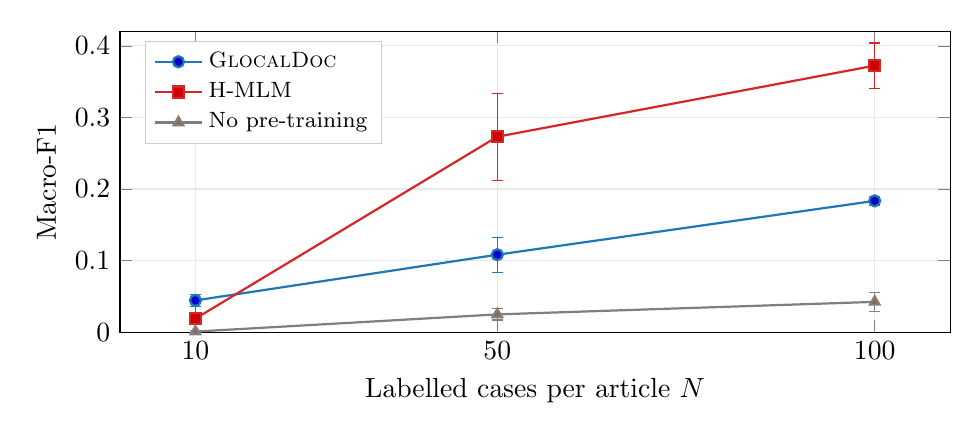
\begin{tikzpicture}
\begin{axis}[
  width=\columnwidth, height=5.4cm,
  xlabel={Labelled cases per article $N$},
  ylabel={Macro-F1},
  xtick={10,50,100}, xmin=0, xmax=110,
  ymin=0, ymax=0.42,
  grid=both, grid style={gray!18},
  legend pos=north west, legend cell align=left,
  legend style={font=\footnotesize, draw=gray!40},
  every axis plot/.append style={thick, mark size=2pt},
]
\addplot+[color=cGlocal, mark=*, error bars/.cd, y dir=both, y explicit]
  coordinates {(10,0.0443) +- (0,0.0086) (50,0.1082) +- (0,0.0243) (100,0.1834) +- (0,0.0060)};
\addlegendentry{\glocal{}}
\addplot+[color=cHmlm, mark=square*, error bars/.cd, y dir=both, y explicit]
  coordinates {(10,0.0189) +- (0,0.0226) (50,0.2730) +- (0,0.0608) (100,0.3723) +- (0,0.0317)};
\addlegendentry{\hmlm{}}
\addplot+[color=cNone, mark=triangle*, error bars/.cd, y dir=both, y explicit]
  coordinates {(10,0.0008) +- (0,0.0013) (50,0.0248) +- (0,0.0079) (100,0.0423) +- (0,0.0133)};
\addlegendentry{No pre-training}
\end{axis}
\end{tikzpicture}
\caption{Macro-F1 against the number of labelled cases per article, with one
standard deviation over five seeds. \glocal{} leads at $N=10$ and has the smallest
spread there; \hmlm{} overtakes it from $N=50$ and widens the gap at $N=100$.}
\label{fig:macro}
\end{figure}

% ---------------------------------------------------------------------------
\section{Results and Analysis}
\label{sec:results}
% ---------------------------------------------------------------------------
Table~\ref{tab:main} reports the test results and Figure~\ref{fig:macro} plots the
macro-F1 against $N$. We read them against the three research questions.

\subsection{RQ1 and RQ2: the advantage is regime-dependent}
There is no single winner. At $N=10$ \glocal{} reaches a macro-F1 of $0.044$ against
$0.019$ for \hmlm{} and $0.001$ for the unpretrained baseline, and the same ordering
holds for micro-F1. From $N=50$ the picture inverts: \hmlm{} reaches $0.273$ against
$0.108$ for \glocal{} at $N=50$, and $0.372$ against $0.183$ at $N=100$. The
hypothesis that a global bottleneck representation helps under scarcity is therefore
confirmed only in the smallest regime, and is contradicted once a moderate amount of
supervision is available.

The most informative quantity at $N=10$ is the variance rather than the mean. The
per-seed scores in Appendix~\ref{app:perseed}, Table~\ref{tab:perseed}, show that
\hmlm{} returns $0.000$ and $0.001$ on two of five seeds at $N=10$, that is, it fails
to learn anything on those runs, while \glocal{} stays in a narrow band between
$0.035$ and $0.057$. The bottleneck behaves as a strong prior. When ten cases per
article are not enough to identify a good linear separator from a high-variance MLM
representation, the compressed representation still supports a usable one, and it
does so consistently. As $N$ grows the prior turns into a handicap, because the same
compression discards lexical detail that the MLM objective preserves and that a
linear head can exploit once it has enough labelled examples to do so. The
unpretrained baseline stays near zero throughout, which confirms that the effects we
measure come from pre-training and not from the architecture or the optimiser.

\subsection{RQ3: collapse and the role of centring}
\glocal{} does not train out of the box on this corpus. Before the centring fix, the
inter-document cosine of the student document code climbed to about $0.99$ within the
first few hundred steps and the run produced the degenerate representation already
visible in the early baseline numbers. Figure~\ref{fig:dynamics} shows the first
epoch after the fix. The collapse metric, defined as the mean pairwise cosine of the
post-predictor document codes over a sliding window, falls from $0.42$ to below
$0.05$ and stays well under the alarm and stop thresholds for the rest of the epoch
(panel a). The centred teacher target has a pairwise cosine near zero throughout,
which is direct evidence that centring absorbs the constant component of the
boilerplate-dominated representation. The bottleneck stays informative: the fraction
of latent dimensions above the free-bits floor rises toward $0.58$ as $\beta$ warms
up, and the mean magnitude of $\mu$ grows in step (panel b). The two document-level
alignment losses decrease over the epoch despite the rising compression weight
(panel c). The uncertainty weighting is active rather than degenerate (panel d): the
log-variance of the compression term grows, which down-weights a loss whose floor is
already handled by free bits, while the local term is up-weighted as the hardest of
the four to satisfy. Without centring none of this happens, and the same
configuration collapses within the first ten percent of training.

\subsection{Document homogeneity}
The centring requirement is a property of the corpus, not of the method in general.
The probe reported in Section~\ref{sec:method}, a median pairwise cosine of $0.9997$
over $200$ documents, quantifies how little the raw encoder distinguishes one
judgment from another. On a corpus whose documents already occupy distinct regions
of the embedding space, the teacher target carries enough variation on its own and
the predictor asymmetry alone would likely suffice. Legal text is at the opposite
extreme, and we expect any non-contrastive document objective to need an explicit
centring or sharpening step on such data.

% ---------------------------------------------------------------------------
% Training dynamics figure (full width)
% ---------------------------------------------------------------------------
\begin{figure*}[t]
\centering
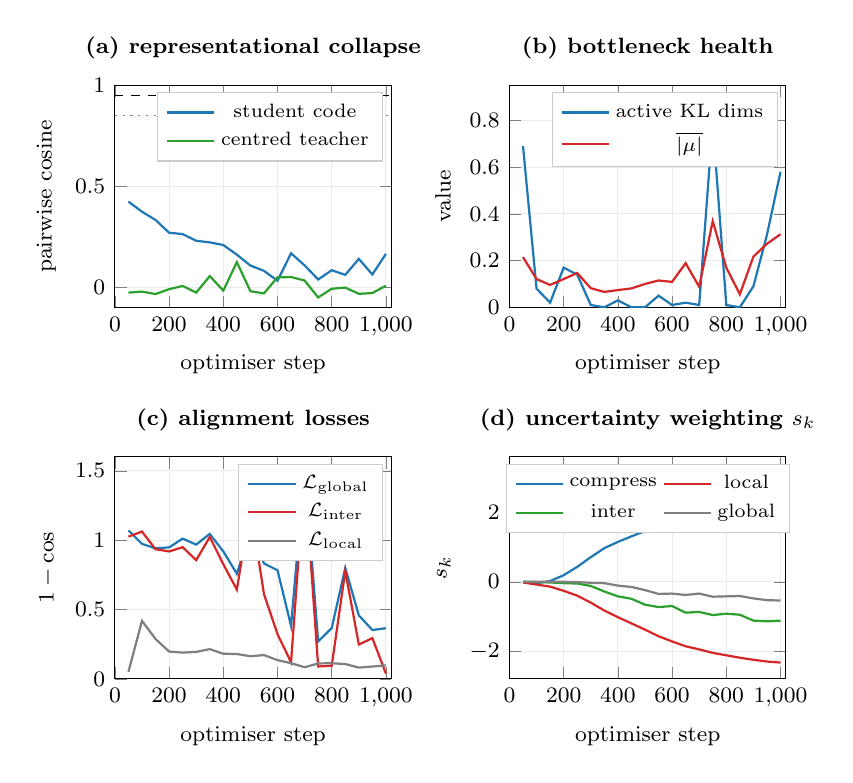
\begin{tikzpicture}
\begin{groupplot}[
  group style={group size=2 by 2, horizontal sep=1.5cm, vertical sep=1.9cm},
  width=0.42\textwidth, height=4.4cm,
  xlabel={optimiser step}, xmin=0, xmax=1020,
  grid=both, grid style={gray!16},
  tick label style={font=\footnotesize},
  label style={font=\footnotesize},
  title style={font=\footnotesize\bfseries},
  legend style={font=\scriptsize, draw=gray!40},
  every axis plot/.append style={thick},
]
% Panel a: collapse
\nextgroupplot[title={(a) representational collapse}, ylabel={pairwise cosine}, ymin=-0.1, ymax=1.0, legend pos=north east]
\addplot[color=cGlocal] coordinates {(50,0.424)(100,0.374)(150,0.333)(200,0.270)(250,0.263)(300,0.230)(350,0.222)(400,0.209)(450,0.161)(500,0.107)(550,0.081)(600,0.032)(650,0.168)(700,0.108)(750,0.038)(800,0.084)(850,0.061)(900,0.140)(950,0.063)(1000,0.165)};
\addlegendentry{student code}
\addplot[color=cAux] coordinates {(50,-0.027)(100,-0.022)(150,-0.034)(200,-0.010)(250,0.006)(300,-0.027)(350,0.055)(400,-0.017)(450,0.124)(500,-0.020)(550,-0.031)(600,0.049)(650,0.050)(700,0.033)(750,-0.051)(800,-0.008)(850,-0.002)(900,-0.033)(950,-0.029)(1000,0.007)};
\addlegendentry{centred teacher}
\addplot[black, dashed, thin] coordinates {(0,0.95)(1020,0.95)};
\addplot[gray, dotted, thin] coordinates {(0,0.85)(1020,0.85)};
% Panel b: bottleneck health
\nextgroupplot[title={(b) bottleneck health}, ylabel={value}, ymin=0, ymax=0.95, legend pos=north east]
\addplot[color=cGlocal] coordinates {(50,0.69)(100,0.08)(150,0.02)(200,0.17)(250,0.14)(300,0.01)(350,0.00)(400,0.03)(450,0.00)(500,0.00)(550,0.05)(600,0.01)(650,0.02)(700,0.01)(750,0.79)(800,0.01)(850,0.00)(900,0.09)(950,0.31)(1000,0.58)};
\addlegendentry{active KL dims}
\addplot[color=cHmlm] coordinates {(50,0.215)(100,0.121)(150,0.096)(200,0.121)(250,0.147)(300,0.082)(350,0.066)(400,0.074)(450,0.081)(500,0.100)(550,0.115)(600,0.109)(650,0.189)(700,0.088)(750,0.369)(800,0.170)(850,0.056)(900,0.217)(950,0.272)(1000,0.313)};
\addlegendentry{$\overline{|\mu|}$}
% Panel c: alignment losses
\nextgroupplot[title={(c) alignment losses}, ylabel={$1-\cos$}, ymin=0, ymax=1.6, legend pos=north east]
\addplot[color=cGlocal] coordinates {(50,1.071)(100,0.973)(150,0.941)(200,0.948)(250,1.011)(300,0.968)(350,1.045)(400,0.919)(450,0.758)(500,1.064)(550,0.832)(600,0.783)(650,0.382)(700,1.522)(750,0.270)(800,0.366)(850,0.800)(900,0.458)(950,0.352)(1000,0.365)};
\addlegendentry{$\mathcal{L}_{\mathrm{global}}$}
\addplot[color=cHmlm] coordinates {(50,1.0252)(100,1.0621)(150,0.9348)(200,0.9185)(250,0.9494)(300,0.8559)(350,1.0227)(400,0.8272)(450,0.6434)(500,1.2423)(550,0.6117)(600,0.3221)(650,0.1197)(700,1.4786)(750,0.0894)(800,0.0945)(850,0.7783)(900,0.2475)(950,0.2939)(1000,0.0380)};
\addlegendentry{$\mathcal{L}_{\mathrm{inter}}$}
\addplot[color=cNone] coordinates {(50,0.0506)(100,0.4183)(150,0.2875)(200,0.1973)(250,0.1891)(300,0.1947)(350,0.2143)(400,0.1812)(450,0.1793)(500,0.1632)(550,0.1717)(600,0.1353)(650,0.1130)(700,0.0838)(750,0.1113)(800,0.1126)(850,0.1068)(900,0.0811)(950,0.0890)(1000,0.0970)};
\addlegendentry{$\mathcal{L}_{\mathrm{local}}$}
% Panel d: UW log-variances
\nextgroupplot[title={(d) uncertainty weighting $s_k$}, ylabel={$s_k$}, ymin=-2.8, ymax=3.6, legend columns=2, legend style={at={(0.5,0.97)}, anchor=north, font=\scriptsize}]
\addplot[color=cGlocal] coordinates {(50,-0.01)(100,-0.04)(150,0.02)(200,0.19)(250,0.43)(300,0.71)(350,0.97)(400,1.15)(450,1.31)(500,1.46)(550,1.60)(600,1.71)(650,1.81)(700,1.88)(750,1.97)(800,2.04)(850,2.11)(900,2.17)(950,2.23)(1000,2.28)};
\addlegendentry{compress}
\addplot[color=cHmlm] coordinates {(50,-0.02)(100,-0.08)(150,-0.14)(200,-0.26)(250,-0.40)(300,-0.60)(350,-0.83)(400,-1.02)(450,-1.20)(500,-1.38)(550,-1.57)(600,-1.72)(650,-1.86)(700,-1.95)(750,-2.05)(800,-2.12)(850,-2.19)(900,-2.25)(950,-2.30)(1000,-2.33)};
\addlegendentry{local}
\addplot[color=cAux] coordinates {(50,0.00)(100,-0.01)(150,-0.02)(200,-0.04)(250,-0.05)(300,-0.12)(350,-0.28)(400,-0.42)(450,-0.49)(500,-0.66)(550,-0.73)(600,-0.70)(650,-0.89)(700,-0.87)(750,-0.96)(800,-0.92)(850,-0.95)(900,-1.12)(950,-1.14)(1000,-1.12)};
\addlegendentry{inter}
\addplot[color=cNone] coordinates {(50,0.00)(100,-0.001)(150,-0.001)(200,0.00)(250,-0.01)(300,-0.03)(350,-0.04)(400,-0.11)(450,-0.15)(500,-0.24)(550,-0.35)(600,-0.34)(650,-0.38)(700,-0.34)(750,-0.43)(800,-0.42)(850,-0.41)(900,-0.48)(950,-0.53)(1000,-0.54)};
\addlegendentry{global}
\end{groupplot}
\end{tikzpicture}
\caption{First epoch of \glocal{} pre-training after the centring fix. (a) The
collapse metric stays far below the alarm ($0.85$, dotted) and stop ($0.95$, dashed)
thresholds, and the centred teacher target has near-zero pairwise cosine. (b) The
bottleneck remains informative as $\beta$ warms up, with the fraction of active
latent dimensions and the mean magnitude of $\mu$ both rising. (c) The
document-level alignment losses decrease despite the growing compression weight. (d)
The uncertainty weighting log-variances separate, which shows the weighting is
active rather than stuck at its uniform initialisation.}
\label{fig:dynamics}
\end{figure*}

% ---------------------------------------------------------------------------
\section{Discussion}
\label{sec:discussion}
% ---------------------------------------------------------------------------
The result that organises the paper is the crossover in Figure~\ref{fig:macro}. A
compression objective and a reconstruction objective produce representations with
different inductive biases, and the better choice depends on how much supervision the
downstream task will receive. Under ten examples per article the compressed
representation is more linearly separable and far more stable, which is exactly what
a low-data practitioner needs. Past fifty examples the reconstruction representation
provides richer features that a linear head can exploit, and the compression that
helped earlier now removes useful signal. Reading the bottleneck as a learned prior
makes both halves of this behaviour expected rather than contradictory.

The stability finding deserves its own emphasis. Mean macro-F1 at $N=10$ is low for
every method, as it must be with ten examples and ten imbalanced labels, but the
spread differs sharply. A method that returns zero on forty percent of seeds is not
usable in a setting where one cannot afford many annotation rounds, and on this axis
\glocal{} is clearly preferable even where the mean gap to \hmlm{} is small.

Several limitations bound these conclusions. We report one pre-training run per
objective, so the variance we measure is over fine-tuning seeds and not over
pre-training randomness; a pre-training seed could move the crossover point. The
backbone is a distilled six-layer encoder and the pre-training is short, which keeps
the experiments affordable but leaves open whether a larger model or a longer
schedule would let the bottleneck retain more of the detail it currently discards.
The stabilisation mechanisms were introduced as a sequence of diagnostic
interventions against observed collapse rather than as a controlled ablation, so we
can state that the combination trains and that centring is the decisive component on
this corpus, but we cannot yet attribute precise contributions to the variance,
covariance, and temporal terms. All results are on a single dataset in a single
legal jurisdiction.

% ---------------------------------------------------------------------------
\section{Conclusion}
% ---------------------------------------------------------------------------
We introduced \glocal{}, a pre-training framework that compresses a corrupted,
partially observed document through an information bottleneck while aligning it to a
momentum teacher at the paragraph, partial-document, and full-document level. On
few-shot classification of ECtHR cases the framework is preferable to a hierarchical
masked language model only in the smallest-data regime, where it is both more
accurate and far more stable across seeds, and it is outperformed once fifty or more
labelled cases per article are available. We traced a representational collapse to
the near-constant teacher target produced by boilerplate-heavy legal text, and
showed that centring the target removes it. Future work should run controlled
ablations of the stabilisation terms, test a decoupled or annealed compression
schedule that preserves more lexical detail at larger $N$, and study whether the
crossover point can be shifted with a larger backbone or a curriculum over the
number of labelled examples.

% ---------------------------------------------------------------------------
\appendices

\section{Loss details}
\label{app:loss}
The compression term is the closed-form Kullback-Leibler divergence between the
diagonal Gaussian posterior $\mathcal{N}(\mu, \mathrm{diag}(\sigma^2))$ and the
standard normal prior, computed from $\log\sigma$ for numerical stability under
bfloat16. The per-dimension free-bits floor replaces each term by its maximum with
$\lambda$, so a dimension contributes no gradient while it uses fewer than $\lambda$
nats. With $\lambda = 0.05$ and a $256$-dimensional latent the floor on the total
divergence is $12.8$ nats, low enough to permit substantial compression while ruling
out a full posterior collapse to the prior. The cosine objectives use
$d(u,v) = 1 - \cos(u,v)$; $\mathcal{L}_{\mathrm{local}}$ flattens the per-document
paragraph matrices before computing the mean cosine, so each student paragraph is
matched to the teacher paragraph at the same position. The uncertainty weighting
follows the homoscedastic form of \cite{kendall2018multi}, where each learned $s_k$
is the log-variance of a Gaussian likelihood and the term $s_k$ acts as a
regulariser that prevents the weights from growing without bound.

\section{Diagnosing collapse}
\label{app:collapse}
The stabilisation mechanisms were added one at a time in response to distinct
failure modes. A shared stop-gradient encoder collapsed because it could satisfy
every alignment loss by becoming input-invariant; replacing it with a separate
momentum teacher encoder and a student-side predictor removed that fixed point and
let the encoder move. The bottleneck then collapsed downstream, with diverse
paragraph vectors mapped to a constant document code; temporal variance and
covariance terms on the document code and on the bottleneck mean addressed this.
Aggressive free bits at $\lambda = 0.5$ over-constrained the mean and were reduced to
$\lambda = 0.05$. The decisive failure was the near-constant teacher target induced
by boilerplate, measured as a median inter-document cosine of $0.9997$, which DINO
centring removed. The first stable epoch is the one shown in
Figure~\ref{fig:dynamics}.

\section{Hyperparameters}
\label{app:hparams}
Table~\ref{tab:hparams} lists the configuration of both pre-training objectives and
the shared fine-tuning procedure.

\begin{table}[t]
\centering
\caption{Configuration. Top: shared. Middle: \glocal{}. Bottom: \hmlm{} and
fine-tuning.}
\label{tab:hparams}
\footnotesize
\begin{tabular}{l l}
\toprule
Setting & Value \\
\midrule
Backbone & DistilRoBERTa-base (6 layers, 768) \\
Max paragraphs / chunk size & 50 / 510 tokens \\
Precision / optimiser & bfloat16 / AdamW \\
Gradient clip & 1.0 \\
\midrule
\glocal{} epochs / eff. batch & 5 / 8 \\
Encoder LR / weights LR & $3\!\times\!10^{-5}$ / $1\!\times\!10^{-2}$ \\
Schedule / warm-up & linear / 10\% \\
EMA rate $\tau$ & 0.996 \\
$\beta$ final / warm-up fraction & 1.0 / 0.25 \\
Free bits $\lambda$ / latent dim & 0.05 nats / 256 \\
Projector / predictor & 256-512-768 / 768-512-768 \\
Variance / covariance weight & 5.0 / 0.04 \\
Variance hinge $\gamma$ & 0.5 \\
Temporal buffer / var / cov & 16 / 25.0 / 1.0 \\
Centre momentum & 0.9 \\
Sentence / span / paragraph mask & 0.20 / 0.15 / 0.30 \\
\midrule
\hmlm{} epochs / eff. batch & 3 / 4 \\
\hmlm{} LR / loss weight & $5\!\times\!10^{-5}$ / 0.5 \\
\hmlm{} mask rate & 0.15 \\
Fine-tune epochs / LR & 10 / $2\!\times\!10^{-5}$ \\
Fine-tune schedule / threshold & cosine, 10\% / 0.5 \\
$N$ / seeds & \{10, 50, 100\} / \{0,\dots,4\} \\
\bottomrule
\end{tabular}
\end{table}

\section{Per-seed results}
\label{app:perseed}
Table~\ref{tab:perseed} gives the macro-F1 of every run. The two zero entries for
\hmlm{} at $N=10$ are the runs that fail to learn, and they account for most of the
high standard deviation reported for that setting in Table~\ref{tab:main}.

\begin{table}[t]
\centering
\caption{Per-seed macro-F1 on the test split.}
\label{tab:perseed}
\footnotesize
\begin{tabular}{l c c c c c c}
\toprule
Method & $N$ & s0 & s1 & s2 & s3 & s4 \\
\midrule
\multirow{3}{*}{No pre.}
 & 10  & 0.000 & 0.000 & 0.000 & 0.001 & 0.003 \\
 & 50  & 0.017 & 0.033 & 0.031 & 0.027 & 0.016 \\
 & 100 & 0.037 & 0.027 & 0.037 & 0.063 & 0.047 \\
\midrule
\multirow{3}{*}{\hmlm{}}
 & 10  & 0.012 & 0.000 & 0.001 & 0.028 & 0.054 \\
 & 50  & 0.265 & 0.287 & 0.291 & 0.178 & 0.344 \\
 & 100 & 0.390 & 0.376 & 0.395 & 0.317 & 0.383 \\
\midrule
\multirow{3}{*}{\glocal{}}
 & 10  & 0.042 & 0.035 & 0.040 & 0.049 & 0.057 \\
 & 50  & 0.093 & 0.094 & 0.151 & 0.103 & 0.101 \\
 & 100 & 0.184 & 0.191 & 0.178 & 0.188 & 0.177 \\
\bottomrule
\end{tabular}
\end{table}

% ---------------------------------------------------------------------------
\bibliographystyle{IEEEtran}
\bibliography{bibliography}

\end{document}
